\section{Third-order spectra and approximation models}
\label{sec:third-order}

\subsection{Frequency axes and a common call pattern}

A two-dimensional spectrum is evaluated at fixed waiting time
\texttt{T}. Supply one-dimensional \texttt{omega1} and \texttt{omega3}
axes, not a pair of meshgrid matrices. Every third-order grid function
returns a complex NumPy array with shape
\begin{equation}
 (N_3,N_1)=(\mathrm{len}(\omega_3),\mathrm{len}(\omega_1)).
\end{equation}
Thus \texttt{S[j, i]} is the response at excitation coordinate
\texttt{omega1[i]} and detection coordinate \texttt{omega3[j]}.
The axes need not have equal lengths.

The full finite-pulse signature is
\par\noindent
\begin{minipage}{\linewidth}
\begin{lstlisting}[style=python]
finite_pulse_spectrum(
    system, pulse1, pulse2, pulse3, omega1, omega3, T, eta,
    pathway="NR", rho0=None, signature=None,
)
\end{lstlisting}
\end{minipage}\par
All arguments before \texttt{pathway} are required. The pulses can be
three distinct \texttt{GaussianPulse} objects; reusing one object is only
a convenience in the tutorial. \texttt{T} is the interval used in
$e^{\mathcal L T}$ and must use the same time unit as the pulse widths.
Use nonnegative waiting times. The convergence parameter \texttt{eta}
from Section~\ref{sec:linear} damps the causal transforms for excitation
and detection and broadens their resolvents; it is not inserted into the
waiting-time propagator.
Physical waiting-time decay comes from $\mathcal L$.

\par\noindent
\begin{minipage}{\linewidth}
\begin{lstlisting}[style=python]
omega1 = np.linspace(0.7, 1.5, 31)
omega3 = np.linspace(0.7, 1.5, 31)
S_NR = pulsus.finite_pulse_spectrum(
    system=system,
    pulse1=pulse, pulse2=pulse, pulse3=pulse,
    omega1=omega1, omega3=omega3,
    T=20.0, eta=0.02, pathway="NR", rho0=rho_ss,
)
assert S_NR.shape == (len(omega3), len(omega1))
\end{lstlisting}
\end{minipage}\par
The functions evaluate the frequency-domain formula directly. They do not
first generate a time-domain grid or apply a numerical Fourier transform.

\subsection{Rephasing, nonrephasing, and explicit field signs}

The convenience aliases resolve as
\begin{equation}
 \mathrm{NR}: (+1,-1,+1),\qquad
 \mathrm{R}: (-1,+1,+1).
\end{equation}
Calling \texttt{pulsus.pathway\_signs("NR")} returns the first tuple.
The arguments correspond to signed field-frequency components at the
three ordered interactions. A tuple is a field-sign sector and does not
isolate a single microscopic ground-state-bleaching, stimulated-emission,
or excited-state-absorption diagram.

\texttt{signature=(s1,s2,s3)} accepts any three entries chosen from
$+1$ and $-1$ and overrides \texttt{pathway}. For example,
\par\noindent
\begin{minipage}{\linewidth}
\begin{lstlisting}[style=python]
signs = pulsus.resolve_signature(
    pathway="R", signature=(1, -1, 1),
)
assert signs == (1, -1, 1)  # Explicit tuple takes precedence.
\end{lstlisting}
\end{minipage}\par
Use the alias alone for ordinary R/NR calculations so that a conflicting
tuple cannot accidentally conceal the intended selection.

These aliases do not change the supplied axes. With the repository's
signed-frequency convention, the NR resonances are near positive
$\omega_1$ and positive $\omega_3$, while R resonances are near negative
$\omega_1$ and positive $\omega_3$. Construct the increasing native R axis
explicitly:
\par\noindent
\begin{minipage}{\linewidth}
\begin{lstlisting}[style=python]
omega1_R = -omega1[::-1]
S_R = pulsus.finite_pulse_spectrum(
    system=system,
    pulse1=pulse, pulse2=pulse, pulse3=pulse,
    omega1=omega1_R, omega3=omega3,
    T=20.0, eta=0.02, pathway="R", rho0=rho_ss,
)
\end{lstlisting}
\end{minipage}\par
Passing \texttt{pathway="R"} with an NR positive axis does not reflect
the spectrum automatically. To display R on a positive excitation axis,
reverse its columns together with the axis: use
\texttt{-omega1\_R[::-1]} and \texttt{S\_R[:, ::-1]}.
Axis reflection alone does not implement experimental phasing or turn
R plus NR into a calibrated absorptive measurement.

\subsection{Five available grid models}

There are five third-order grid models. Four form a useful approximation
ladder; a full-interaction impulsive molecular reference is also supplied:
\begin{description}
 \item[A: \texttt{finite\_pulse\_spectrum}]
 Full molecular interaction and operator-valued finite-Gaussian dressing.
 Field signs select pulse components without restricting $\mathcal V$.
 \item[B: \texttt{finite\_pulse\_rwa\_spectrum}]
 The same finite-pulse operator dressing, with each interaction replaced
 by $\mathcal V_+$ or $\mathcal V_-$ according to its field sign.
 \item[C: \texttt{short\_pulse\_rwa\_spectrum}]
 RWA molecular response multiplied by scalar Gaussian spectral
 amplitudes; operator-valued intrapulse dressing is omitted.
 \item[D: \texttt{impulsive\_rwa\_spectrum}]
 RWA molecular response without finite pulse filtering or field
 prefactors.
 \item[Full impulsive reference: \texttt{impulsive\_spectrum}]
 Complete interaction at all three steps, without pulse dressing or
 field prefactors. It has no \texttt{pathway} or \texttt{signature}
 argument.
\end{description}
Models B and C share A's signature. D and the full impulsive reference use
\par\noindent
\begin{minipage}{\linewidth}
\begin{lstlisting}[style=python]
impulsive_rwa_spectrum(
    system, omega1, omega3, T, eta,
    pathway="NR", rho0=None, signature=None,
)
impulsive_spectrum(
    system, omega1, omega3, T, eta, rho0=None,
)
\end{lstlisting}
\end{minipage}\par
The RWA models require both dipole components. The full models need only
the complete dipole. The corresponding \texttt{\_signal} functions have
the same high-level arguments with scalar coordinates and return one
complex number; \texttt{\_response} functions take the matrices and
individual pulse parameters directly. For B, the callable scalar names
\texttt{pulsus.finite\_pulse\_rwa\_signal} and
\texttt{pulsus.finite\_pulse\_rwa\_response} exist even though the
release's \texttt{\_\_all\_\_} list omits those two entries. Prefer
\texttt{import pulsus} and qualified names over wildcard imports.

\subsection{A controlled comparison}

Compare models at identical states, frequency coordinates, waiting time,
and \texttt{eta}. With the RWA-capable tutorial system:
\par\noindent
\begin{minipage}{\linewidth}
\begin{lstlisting}[style=python]
grid = dict(system=system, omega1=omega1, omega3=omega3,
            T=20.0, eta=0.02, rho0=rho_ss)
fields = dict(pulse1=pulse, pulse2=pulse, pulse3=pulse,
              pathway="NR")
A = pulsus.finite_pulse_spectrum(**grid, **fields)
B = pulsus.finite_pulse_rwa_spectrum(**grid, **fields)
C = pulsus.short_pulse_rwa_spectrum(**grid, **fields)
D = pulsus.impulsive_rwa_spectrum(**grid, pathway="NR")
M_full = pulsus.impulsive_spectrum(**grid)
\end{lstlisting}
\end{minipage}\par
The complete example \texttt{examples/manual/03\_third\_order\_models.py}
illustrates A--D for both NR and R. The $A-B$ difference isolates the effect of
the molecular RWA within the same finite-pulse construction. The $B-C$
difference measures replacing operator dressing by scalar field factors
within the RWA. A comparison of $C$ to $D$ must account for the field
prefactors: $D$ is a molecular response rather than the polarization
produced by the specified Gaussian pulses.

More explicitly, the short-pulse expression uses
\[
C(\omega_3,\omega_1)=
E_3^{(s_3)}(\omega_3)E_2^{(s_2)}(-\omega_1)
E_1^{(s_1)}(\omega_1)D(\omega_3,\omega_1).
\]
The minus sign in the second pulse's frequency argument is part of this
convention; do not replace it with $+\omega_1$ when constructing the
expression manually.

For pulse signs $s_k$, define
\begin{equation}
 c_k=\frac{E_{0k}}{2}\sqrt{2\pi}\,\sigma_k e^{is_k\phi_k}.
\end{equation}
A flat-envelope impulsive comparison on the finite-pulse amplitude scale
uses $(c_1c_2c_3)D$. For the equal-pulse NR example,
\par\noindent
\begin{minipage}{\linewidth}
\begin{lstlisting}[style=python]
signs = pulsus.pathway_signs("NR")
area_factor = np.prod([
    pulsus.gaussian_prefactor(
        sigma=pulse.sigma, E0=pulse.E0,
        phase=pulse.phase, sign=s,
    ) for s in signs
])
D_on_field_scale = area_factor * D
\end{lstlisting}
\end{minipage}\par
This restores the signed Gaussian prefactors, not the frequency-dependent
filtering of C. At fixed peak field, reducing all widths to zero also
reduces $c_1c_2c_3$ to zero. A statement about the impulsive limit must
therefore specify fixed peak field, fixed area, or removal of prefactors.

\begin{figure}[!htbp]
\centering
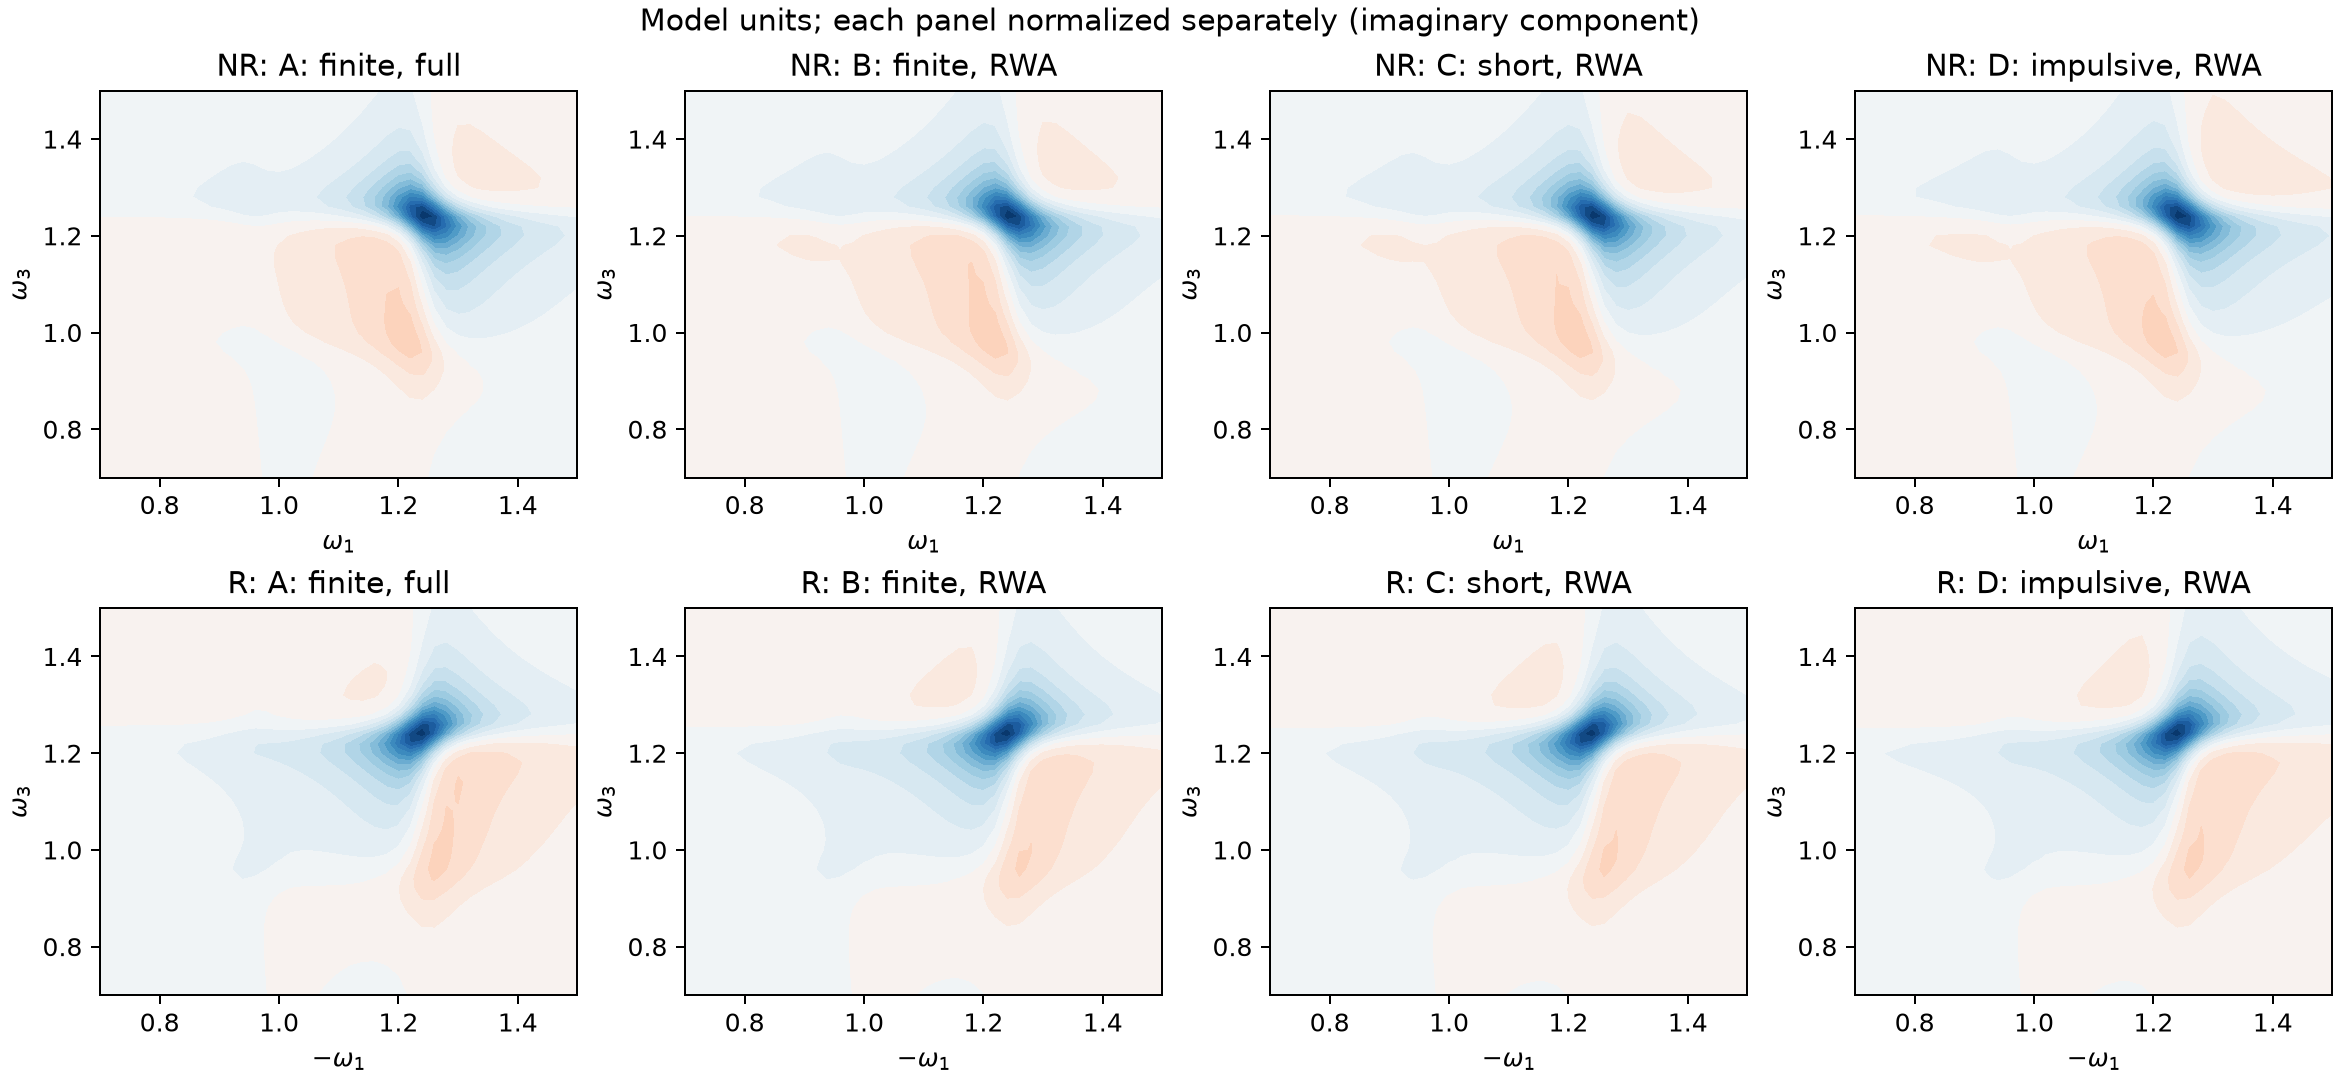
\includegraphics[width=\linewidth]{figures/third_order_models.png}
\caption{A--D for NR (top) and R (bottom), displayed against positive
spectroscopic excitation coordinates. Every panel shows the imaginary
component normalized separately to its maximum absolute value; the
shared red/blue range is $[-1,1]$. This visualization does not preserve
relative amplitudes. The example uses unit Gaussian prefactors at zero pulse phase, $\sigma=1.25$, $T=20$ and $\eta=0.02$.}
\label{fig:third-order-models}
\end{figure}

\subsection{Interpreting plots and convergence}

The array contains a complex response. A contour of its imaginary part
can have positive and negative lobes; its sign is not a population
probability. Interference, field phases, detection convention, and the
selected quadrature all contribute. A single colored lobe should not be
assigned to one microscopic diagram solely from this plot.

Normalized contour plots help inspect shape, but retain the original
complex arrays for amplitude comparisons. Refine axes until the features
used in the analysis are stable; grid agreement does not remove
approximation error. Vary pulse width and \texttt{eta} independently,
and distinguish physical broadening in $\mathcal L$ from convergence
broadening. The finite-pulse APIs implement the repository's ordered
Gaussian dressing model; the word ``finite'' does not turn this into a
general numerical propagation of an arbitrary overlapping pulse train.
